\documentclass[12pt]{article}
\usepackage{caption}
\usepackage{graphicx}
\usepackage{hyperref}
\hypersetup{%
    pdfborder = {0 0 0}
}
\hypersetup{
    colorlinks,
    citecolor=blue,
    filecolor=blue,
    linkcolor=blue,
    urlcolor=blue
}
\renewcommand{\familydefault}{\sfdefault}
\renewcommand{\captionfont}{\small}

\author{Bernd Porr}
\title{Induktives Lernen anhand neuronaler Netze}

\begin{document}

\maketitle

\section{Induktives lernen}
Bekannt ist ein Datensatz $\vec{x}_1, \ldots, \vec{x}_N$, der mit einer unbekannten Funktion $\vec{y}=f(\vec{x})$ in einen Datensatz $\vec{y}$
ueberfuerhrt wird. Das Ziel ist es, die Funktion $f$ iterativ mit Hilfe von Beispielen $\vec{x},\vec{y}$ zu lernen.

In den folgenden Abschnitten wird die Funktion $f$ durch immer komplexere neuronale Netzwerke gelernt und approximiert.

\section{Lineares Neuron}

\begin{figure}[!hbt]
\begin{center}
\mbox{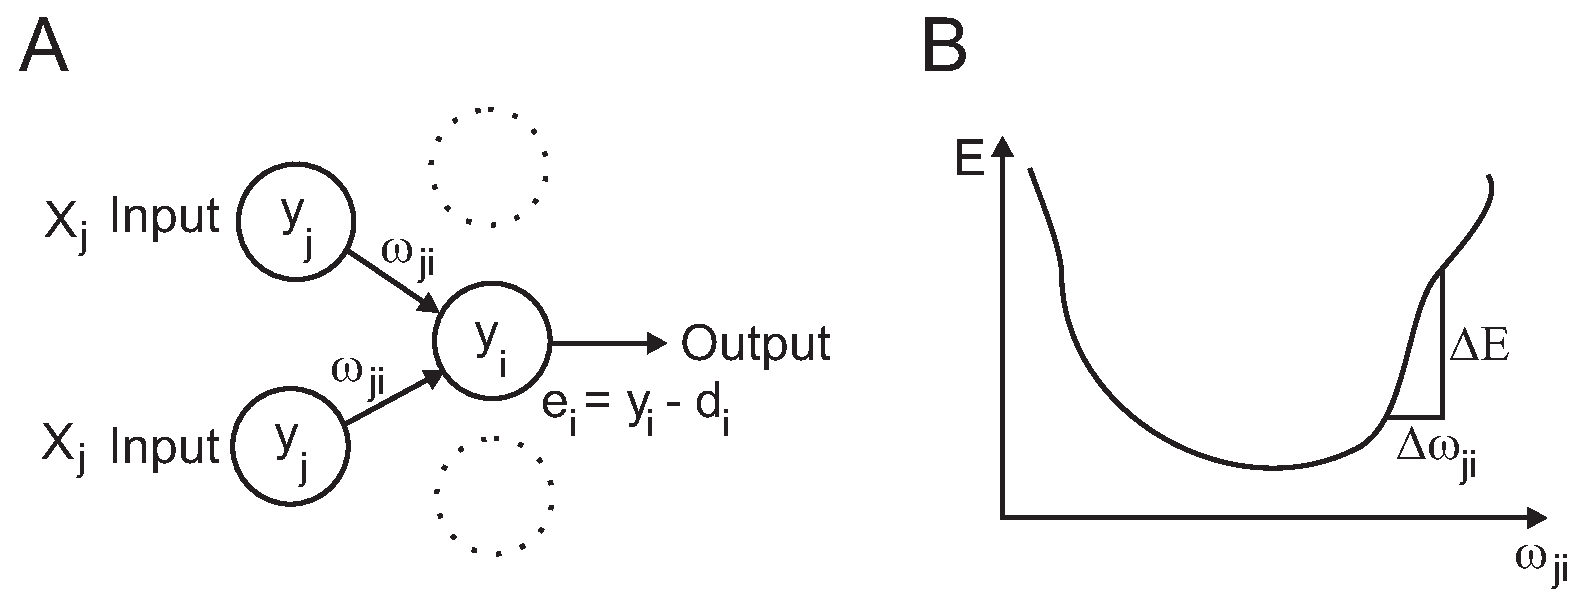
\includegraphics[width=\textwidth]{one_layer}}
\end{center}
\caption{Einfaches lineares Neuron
\label{one_layer}}
\end{figure}

Abb.~\ref{one_layer}A zeigt ein einfaches lineares Neuron in einer
einzigen Schicht. Die Aktivitaet des neurons ist $y$ und hat einen
Index fuer dessen Position in der Schicht, wobei der index $i$ hier
die Ausgangsschicht repreaesentiert. Die Eingangsaktivitaet $x_j =
y_j$ wird mit $\omega_{ji}$ gewichtet und dann zum Ausgangssignal
$y_i$ summiert:
\begin{equation}
  y_i(n) = \sum_j y_j(n) w_{ji} \label{linear_sum}
\end{equation}
Die funktion $f$ ist hier also eine einfache lineare Kombination von den Eingangssignalen, wobei
die Gewichte $\omega_{ji}$ gelernt werden muessen, um die spezifische Funktion $f$ zu approximieren.

Gelernt werden soll eine bestimmte Ausgangsaktivitaet in Abhanengigkeit von einer Eingangsaktivitaet.
Das wird erreicht, indem ein Fehler $e_i$ am Ausgang jedes Neurons etabliert wird, der dann die Gewichte $w_{ji}$
schrittweise dorthin beweget, dass er im mittel Null wird:
\begin{equation}
  e_i = y_i - d_i \label{output_error}
\end{equation}
wobei $d_i$ der gewuenschte Ausgangswert ist und $y_i$ der Aktuelle.
Ziel des Lernen ist es, dass das quadratische Mittel null wird:
\begin{equation}
  E = \frac{1}{2} e^2
\end{equation}

Der zentrale Trick ist nun, die Partielle Ableitung in Abhaengigkeit vom Fehler $E$ zu nehmen
und damit die Gewichte zu veraendern:
\begin{eqnarray}
  \Delta\omega_{ji} & = & - \mu \frac{\partial E}{\partial \omega_{ji}} \label{graddes} \\
  \omega_{ji} & \leftarrow & \omega_{ji} + \Delta\omega_{ji}
\end{eqnarray}
Warum macht das Sinn? In Abb.~\ref{one_layer}B ist die Abhaengigkeit von einem Gewicht
$\omega_{ji}$ gezeigt. wenn in diesem Beispiel das Gewicht etwas erhoeht wird, dann
wird der Fehler $E$ groesser also war die Erhoehung kontraproduktiv und es ist besser,
das Gewicht zu verringern. Wenn aber umgekehrt eine Erhoehung von $\omega_{ji}$ eine
Verringerung von E bewirkt, dann ist das Vorteilhaft also kann man das Gewicht erhoehen.
Iterativ wird also der Fehler verringert.

Als naechsten Schritt muss nun die Lernregel hergeleitet werden. Das geschieht, indem
mein einfach Gl.~\ref{linear_sum} in Gl.~\ref{graddes} einsetzt und die Partiellen Ableitungen
durchfuehrt:
\begin{eqnarray}
  \Delta\omega_{ji}
   & = & - \mu \frac{1}{2} \frac{\partial ( d_i(n) - y_i(n) )^2 }{\partial \omega_{ji}} \\
   & = & - \mu \frac{1}{2} \frac{\partial ( d_i(n) - \left( \sum_j y_j(n) w_{ji} \right)^2 }{\partial \omega_{ji}} \\
   & = & - \mu \underbrace{\frac{\partial E}{\partial y_i}}_{-e_i(n)} \underbrace{\frac{\partial y_i}{\partial \omega_{ji}}}_{y_j(n)} \label{chainrule}\\
  & = & \mu \underbrace{\left(d_i(n) - \sum_j y_j(n) w_{ji}\right)}_{e_i(n)} \cdot y_j(n) \\
  & = & \mu \cdot e_i(n) \cdot y_j(n)
\end{eqnarray}

\section{Mehrschichtiges lineares Netzwerk}
\begin{figure}[!hbt]
\begin{center}
\mbox{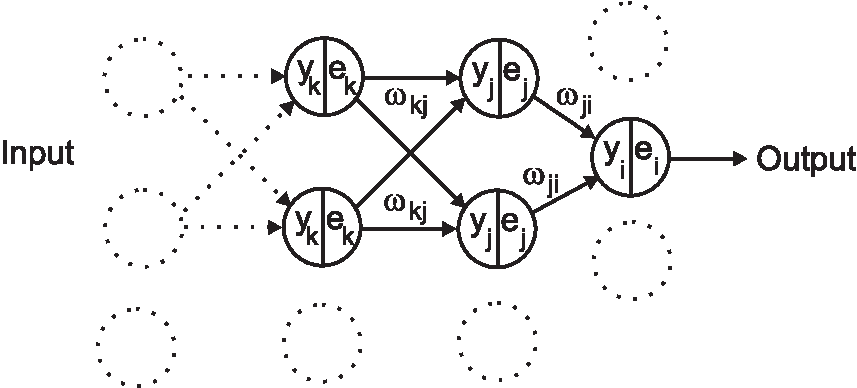
\includegraphics[width=\textwidth]{multi_layer}}
\end{center}
\caption{Mehrschichtiges Feedforward Netz
\label{multi_layer}}
\end{figure}

Abb.~\ref{multi_layer} zeigt nun ein Netzwerk mit mehreren
Schichten. Wie das Signal vom Eingang zum Ausgang durch die
verschiedenen Schichten laeuft, ist einfach auszurechnen. Auch der
Fehler $e_i$ in der Ausgangsschicht kann weiterhin einfach als
Differenz zwischen $y_i$ und $d_i$ ausgerechnet werden (siehe
Gl.~\ref{output_error}). Das Problem ist, wie die \textsl{internen} Fehler
$e_j$ und $e_k$ ausgerechnet werden koennen.
Der interne Fehler fuer $\omega_{kj}$ ist erstmal genauso definiert wie der Fehler
am Ausgang (siehe Gl.~\ref{chainrule}):
\begin{equation}
  \frac{\partial E}{\partial \omega_{kj}} = \underbrace{\frac{\partial E}{\partial y_j}}_\textrm{Trick!} \frac{\partial y_j}{\partial \omega_{kj}}
  \label{gradint}
\end{equation}
Der Trick ist nun diesen Term mit Hilfe von $y_i$ auszudruecken und dann einfach die beiden Terme mit Gl.~\ref{linear_sum} und Gl.~\ref{chainrule} zu identifizieren:
\begin{equation}
  \frac{\partial E}{\partial y_j} = \sum_i \underbrace{\frac{\partial E}{\partial y_i}}_{-e_i} \cdot \underbrace{\frac{\partial y_i}{\partial y_j}}_{\omega_{ji}} \label{dltrick}
\end{equation}
Gl.~\ref{dltrick} wieder in Gl.~\ref{gradint} substituiert gibt dann:
\begin{equation}
  \frac{\partial E}{\partial \omega_{kj}} = - \left( \sum_i e_i \omega_{ji} \right) \frac{\partial y_j}{\partial \omega_{kj}}
  \label{gradint}
\end{equation}
mit
\begin{equation}
y_j = \sum_k y_k(n) w_{kj}
\end{equation}
und fuert zu:
\begin{eqnarray}
  \frac{\partial E}{\partial \omega_{kj}} & = & - \left( \sum_i e_i \omega_{ji} \right) \underbrace{\frac{\partial y_j}{\partial \omega_{kj}}}_{y_k} \\
                                         & = & - \left( \sum_i e_i \omega_{ji} \right) y_k
\end{eqnarray}
Die Aenderung des Gewichtes $\omega_{kj}$ folgt dann folgender Gleichung:
\begin{equation}
\Delta\omega_{kj} = \mu \cdot y_k \cdot \underbrace{\sum_i e_i \omega_{ji}}_{e_j}
\end{equation}
Wobei nun $e_j$ der interne Error ist und damit es moeglich ist, rueckwaerts vom Ausgang zum Eingang alle Fehler zu berechnen.

\begin{figure}[!hbt]
\begin{center}
\mbox{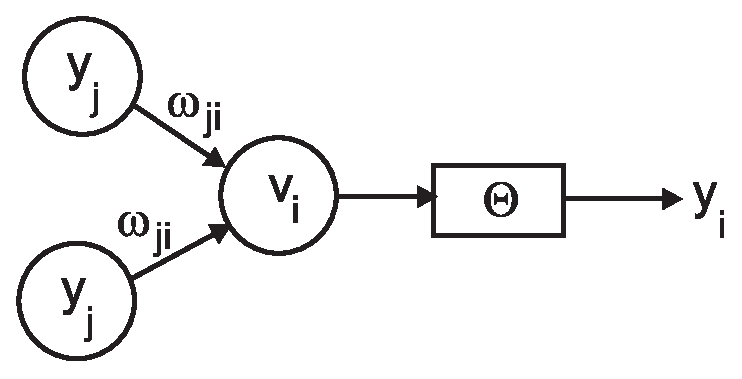
\includegraphics[width=0.5\textwidth]{nonlin}}
\end{center}
\caption{Neuron mit nichtlinearer Characteristik
\label{nonlin}}
\end{figure}

\section{Nicht-lineare Netzwerke}
Nur wenn Netzwerke nicht-linear sind, machen tiefere Schichten einen Sinn, da jedes lineare Netzwerk immer auf eine Schicht reduziert werden kann.
Erst die Nichtlinearitaet rechtfertigt ``Deep'' Netzwerke.
Abb.~\ref{nonlin} zeigt ein Neuron von einem Netzwerk, wo die lineare Summe dann durch eine Nichtlinearitaet geschickt wird.
\begin{equation}
  y_i(n) = \Theta(\underbrace{\sum_j y_j(n) w_{ji}}_{v_i}) \label{linear_sum}
\end{equation}
Was aendert sich in diesem Fall an den Lernregeln? Sehr wenig. Wenn man sich Gl.~\ref{chainrule} ansieht, merkt man, dass einfach
ein weiterer Term durch die Kettenregel hinzukommt:
 \begin{equation}
 \frac{\partial E}{\partial \omega_{ji}}  = \frac{\partial E}{\partial y_i} \underbrace{\frac{\partial y_i}{\partial v_i}}_{\Theta^\prime} \frac{\partial v_i}{\partial \omega_{ji}}
 \end{equation}
 wo $\Theta^\prime$ einfach die Ableitung der nicht-linearen Aktivierungsfunktion $\Theta$ ist. Das heisst, dass der Fehler fuer die
 Ausgangsschicht jetzt folgendermassen ausgerechent wird:
\begin{equation}
  \Delta\omega_{ji} = \mu \cdot \Theta^\prime(y_i) \cdot y_j \cdot e_i 
\end{equation}
und der interne Fehler:
\begin{equation}
\Delta\omega_{kj} = \mu \cdot \Theta^\prime(y_j) \cdot y_k \cdot \underbrace{\sum_i e_i \omega_{ji}}_{e_j} 
\end{equation}







\end{document}
